\documentclass[12pt]{article}

\usepackage[english]{babel}                 %%%%%%%%%%%%%    (EDIT LANGUAGE)
\usepackage{Custom}                         %%%%%%%%%%%%%    (EDIT NAMES+ABSTRACT)
\usepackage{AuxiliaryFiles/AuxiliaryFiles}  %%%%%%%%%%%%%    (DO NOT EDIT)
\usepackage{Custom-2}                       %%%%%%%%%%%%%%   (EDIT)

\begin{document}
\newcommand\IndexYes{1}
    %%%%%%%%%%%%%%%%%%   (IF A TABLE OF CONTENTS IS NOT NEEDED, CHANGE 1 TO 0)
\newcommand\AbstractYes{1}
    %%%%%%%%%%%%%%%%%%   (IF AN ABSTRACT IS NOT NEEDED, CHANGE 1 TO 0)
% !TEX root = ../../ArticleTemplate.tex
%%%%%%%%%%%%%%%%%%%%%%%%%%%%%%%%%%%%%%%%%%%%%%%%%%%%%%%%%%%%%%%%%%%%%%%%%%%%%%%%%%
\title{\Title}
\author{\Author\\ \EMail}
\date{\Date}
\maketitle
\ifnum\AbstractYes=1
\UnderlineBox{\Abstract}
\fi   %%%%%%%%%%%%%%%%%%        (EDIT TITLEPAGE)


% !TEX root = ../ArticleTemplate.tex
%%%%%%%%%%%%%%%%%%%%%%%%%%%%%%%%%%%%%%%%%%%%%%%%%%%%%%%%%%%%%%%%%%%%%%%%%%%%%%%%%%
%%%%%%%% TABLE OF CONTENTS
\ifnum\IndexYes=1
\setlength\columnsep{40pt}
\makeatletter
\renewcommand{\tableofcontents}{
{
\begin{multicols}{2}
		\fontsize{10}{14.4}\selectfont 
	\@starttoc{toc}
\end{multicols}
}}
\makeatother

\contentsmargin{0cm}
	% TOC Section
\titlecontents{section}[0pc]
{\addvspace{8pt}\normalsize\bfseries\thecontentslabel}{\hspace{.5cm}}{}
{\tiny\color{black!50}\;\;\dotfill\;\normalsize\bfseries\color{black}\PageName\, \thecontentspage}
    % TOC Subsection
\titlecontents{subsection}[.5pc]
{\addvspace{1pt}\bfseries\thecontentslabel\normalfont}{\hspace{.25cm}}{}
{\tiny\color{black!50}\;\;\dotfill\;\small\color{black}\PageName\, \thecontentspage}
	% TOC Subsubsection
\titlecontents{subsubsection}[1pc]
{\addvspace{1pt}\bfseries\thecontentslabel\normalfont}{\hspace{.25cm}}{}
{\tiny\color{black!50}\;\;\dotfill\;\small\color{black}\PageName\, \thecontentspage}
{
    \let\cleardoublepage\relax
	\renewcommand\contentsname{}
    \begin{minipage}[r]{.95\textwidth}\raggedleft
    \vspace{.5cm}
    \Large\bfseries\ContentsName
	\vspace{.5cm}
    \end{minipage}

	\tableofcontents
	\vspace{.25cm}
}
\fi  %%%%%%%%%%%%%%%%%%           (DO NOT EDIT)

% !TEX root = ../ArticleTemplate.tex
%%%%%%%%%%%%%%%%%%%%%%%%%%%%%%%%%%%%%%%%%%%%%%%%%%%%%%%%%%%%%%%%%%%%%%%%%%%%%%%%%%

\section*{\IntroductionName}
\addcontentsline{toc}{section}{\IntroductionName}
                    %%%%%%%%%%%%%%%%%%%%%%%%%%%%                  (EDIT BELOW)
This is the document that has a lot of commonly used environments and notes. When you want to see how to type
them out, use ``Ctrl + Leftclick''. For the environment, most are typed out as: Environment, and their corresponding appearance. For example: \newpage
\begin{verbatim}
\begin{Le}{}{Label}
    This is the Lemma
\end{Le}
\end{verbatim}
\begin{Le}{}{Label}
    This is the Lemma
\end{Le}      %%%%%%%%%%%%%%%%%%     (EDIT INTRODUCTION)

% !TEX root = ../ArticleTemplate.tex
%%%%%%%%%%%%%%%%%%%%%%%%%%%%%%%%%%%%%%%%%%%%%%%%%%%%%%%%%%%%%%%%%%%%%%%%%%%%%%%%%%
\section{Environments}
\subsection{Theorems and Proofs}
\fbox{\parbox{.8\textwidth}{
 have edited the commands in this and the following sections. Now, two new arguments are required. The first is an additional description in the environment’s title (especially useful for remarks and examples). The second is the label of the environment, which is needed for cross-references. Both arguments may be left empty.}}
\vspace{.25cm}

\begin{verbatim}
\begin{The}{Additional title}{Label}
\lipsum[2]
\end{The}
\end{verbatim}

\begin{The}{Additional title}{Label}
\lipsum[2]
\end{The}
%%%%%%%%%%%%%%%%%%%%%%%%%%%%%%%%%%%
\begin{verbatim}
\begin{Proof}
\lipsum[2]
\end{Proof}
\end{verbatim}

\begin{Proof}
\lipsum[2]
\end{Proof}
%%%%%%%%%%%%%%%%%%%%%%%%%%%%%%%%%%%
\begin{verbatim}
\begin{Pro}{}{Label}
\lipsum[1]
\end{Pro}
\end{verbatim}

\begin{Pro}{}{Label}
\lipsum[1]
\end{Pro}
%%%%%%%%%%%%%%%%%%%%%%%%%%%%%%%%%%%
\begin{verbatim}
\begin{Le}{}{Label}
\lipsum[2]
\end{Le}
\end{verbatim}

\begin{Le}{}{Label}
\lipsum[2]
\end{Le}
%%%%%%%%%%%%%%%%%%%%%%%%%%%%%%%%%%%
\begin{verbatim}
\begin{Co}{}{Label}
\lipsum[2]
\end{Co}
\end{verbatim}

\begin{Co}{}{Label}
\lipsum[2]
\end{Co}
%%%%%%%%%%%%%%%%%%%%%%%%%%%%%%%%%%%%%%%%%%%%%%%%%%%%%%%%%%%%%%%%%%%%%%%%%%%%
\subsection{Definitions, Examples, Remarks}
\begin{verbatim}
\begin{De}{}{Label}
\lipsum[2]
\end{De}
\end{verbatim}

\begin{De}{}{Label}
\lipsum[2]
\end{De}
%%%%%%%%%%%%%%%%%%%%%%%%%%%%%%%%%%%
\begin{verbatim}
\begin{Exa}{}{Label}
\lipsum[8]
\end{Exa}
\end{verbatim}

\begin{Exa}{}{Label}
\lipsum[8]
\end{Exa}
%%%%%%%%%%%%%%%%%%%%%%%%%%%%%%%%%%%
\begin{verbatim}
\begin{Rmk}{}{Label}
\lipsum[2]
\end{Rmk}
\end{verbatim}

\begin{Rmk}{}{Label}
\lipsum[2]
\end{Rmk}
%%%%%%%%%%%%%%%%%%%%%%%%%%%%%%%%%%%
\paragraph*{}
There are similar commands to create a Theorem, Proposition... without numbering. Here, only a new argument is required for an additional description in the title. For instance:

\begin{verbatim}
\begin{Pro*}{}
\lipsum[2]
\end{Pro*}
\end{verbatim}

\begin{Pro*}{}
\lipsum[2]
\end{Pro*}



\subsection{Description, itemize, enumerate}
\paragraph*{} \underline{Description with boxed labels}
\begin{verbatim}
\begin{description}
  \item[\boxlabel{Label 1}{1.5cm}]
        \lipsum[1]
  \item[\boxlabel{Label 2 with a very long comment}{4cm}]
        \lipsum[2]
\end{description}
\end{verbatim}

\begin{description}
  \item[\boxlabel{Label 1}{1.5cm}]
        \lipsum[1]
  \item[\boxlabel{Label 2 with a very long comment}{4.2cm}]
         \lipsum[2]
\end{description}
%%%%%%%%%%%%%%%%%%%%%%%%%%%%%%%%%%%

\paragraph*{} \underline{Description}
\begin{verbatim}
\begin{description}
\item[Label 1] \lipsum[1]
\item[Label 2] \lipsum[2]
\end{description}
\end{verbatim}

\begin{description}
\item[Label 1] \lipsum[1]
\item[Label 2] \lipsum[2]
\end{description}
%%%%%%%%%%%%%%%%%%%%%%%%%%%%%%%%%%%

\paragraph*{} \underline{Itemize}
\begin{verbatim}
\begin{itemize}
    \item \lipsum[2]
    \item \lipsum[2]
    \item \lipsum[2]
\end{itemize}
\end{verbatim}

\begin{itemize}
    \item \lipsum[2]
    \item \lipsum[2]
    \item \lipsum[2]
\end{itemize}
%%%%%%%%%%%%%%%%%%%%%%%%%%%%%%%%%%%

\paragraph*{} \underline{Enumerate}
\begin{verbatim}
\begin{enumerate}
    \item \lipsum[2]
    \item \lipsum[2]
\end{enumerate}
\end{verbatim}

\begin{enumerate}
    \item \lipsum[2]
    \item \lipsum[2]
\end{enumerate}
%%%%%%%%%%%%%%%%%%%%%%%%%%%%%%%%%%%





\subsection{Margin Notes}
	\lipsum[2]
	\note{Margin note\\
    \text{$\setminus$note\{Note\}}}
	\begin{Rmk}{}{}
    \lipsum[2]
    \note{Margin note}
    \lipsum[2]
    \end{Rmk}
	\lipsum[2]
    \begin{Proof}
    \lipsum[2]
    \sub
    \expl{$\setminus$sub\\
    Different colour\\ to explain a step\\ in a proof\\[2pt] \text{$\setminus$expl\{\#1\}}}
	\lipsum[2]
    \end{Proof}
%%%%%%%%%%%%%%%%%%%%%%%%%%%%%%%%%%%

\subsection{Hypertext links, quotes, indices, urls}\label{Label}
\paragraph*{}
We obtain a hypertext link with
\begin{verbatim}
    \label{Label}
\end{verbatim}
\noindent and we call it with
\begin{verbatim}
    \ref{Label}
\end{verbatim}
Result: Section \ref{Label}

\fbox{\parbox{.8\textwidth}{
Now, to obtain the corrected reference for a theorem, a proposition, a lemma, a corollary, a definition, a example, we must use the second argument in the environments defined as above. Each environment as a key word to write before the effective label. Here there are the key words for each environment: we use as examples the callings of these environments used in the previous sections.}}

\begin{center}
\begin{tabular}{c|c}
Theorem \text{$\setminus$the:Label} & Theorem \ref{the:Label}\\
Proposition \text{$\setminus$pro:Label} & Proposition \ref{pro:Label} \\
Lemma \text{$\setminus$le:Label} & Lemma \ref{le:Label}\\
Corollary \text{$\setminus$co:Label} & Corollary \ref{co:Label}\\
Definition \text{$\setminus$de:Label} & Definition \ref{de:Label}\\
Example \text{$\setminus$exa:Label} & Example \ref{exa:Label}\\
Remark \text{$\setminus$rmk:Label} & Remark \ref{rmk:Label}
\end{tabular}
\end{center}

\paragraph*{}
We quote a book in the bibliography with
\begin{verbatim}
    \cite{LabelBook}
\end{verbatim}
Result: \cite{LabelBook}

\paragraph*{}
We add new elements in the analytic index with
\begin{verbatim}
    \index{Index}
        \index{IndexSecondVoice}
    \index{Index!ThirdVoice}
    \index{Index!ThirdVoice!Part 1}
    \index{Index!ThirdVoice!Part 2}
\end{verbatim}
The result of this two commands is shown in the analytic index at the end of the document.
    \index{Index}
        \index{IndexSecondVoice}
    \index{Index!ThirdVoice}
    \index{Index!ThirdVoice!Part 1}
    \index{Index!ThirdVoice!Part 2}

\paragraph*{}
We create URL links with
\begin{verbatim}
    \url{https://mattiapuddu25.github.io/main/index.html}
\end{verbatim}
Result: \url{https://mattiapuddu25.github.io/main/index.html}          %%%%%%%%%%%%%%%%%%         (EDIT CHAPTERS)
% !TEX root = ../ArticleTemplate.tex
%%%%%%%%%%%%%%%%%%%%%%%%%%%%%%%%%%%%%%%%%%%%%%%%%%%%%%%%%%%%%%%%%%%%%%%%%%%%%%%%%%
\section{New commands}

\Minipage{.4}{\begin{longtable}{r|r|r}
$\setminus$A& $\setminus$AA & $\setminus$AAA    \\\hline\\[-5pt]
$\A$ & $\AA$ & $\AAA$\\[0.1cm]
$\B$ & $\BB$ & $\BBB$\\[0.1cm]
$\C$ & $\CC$ & $\CCC$\\[0.1cm]
$\D$ & $\DD$ & $\DDD$\\[0.1cm]
$\E$ & $\EE$ & $\EEE$\\[0.1cm]
$\F$ & $\FF$ & $\FFF$\\[0.1cm]
$\G$ & $\GG$ & $\GGG$\\[0.1cm]
$\H$ & $\HH$ & $\HHH$\\[0.1cm]
$\I$ & $\II$ & $\III$\\[0.1cm]
$\J$ & $\JJ$ & $\JJJ$\\[0.1cm]
$\K$ & $\KK$ & $\KKK$\\[0.1cm]
$\L$ & $\LL$ & $\LLL$\\[0.1cm]
$\M$ & $\MM$ & $\MMM$\\[0.1cm]
$\N$ & $\NN$ & $\NNN$\\[0.1cm]
$\O$ & $\OO$ & $\OOO$\\[0.1cm]
$\P$ & $\PP$ & $\PPP$\\[0.1cm]
$\Q$ & $\QQ$ & $\QQQ$\\[0.1cm]
$\R$ & $\RR$ & $\RRR$\\[0.1cm]
$\S$ & $\SS$ & $\SSS$\\[0.1cm]
$\T$ & $\TT$ & $\TTT$\\[0.1cm]
$\U$ & $\UU$ & $\UUU$\\[0.1cm]
$\V$ & $\VV$ & $\VVV$\\[0.1cm]
$\W$ & $\WW$ & $\WWW$\\[0.1cm]
$\X$ & $\XX$ & $\XXX$\\[0.1cm]
$\Y$ & $\YY$ & $\YYY$\\[0.1cm]
$\Z$ & $\ZZ$ & $\ZZZ$\\[0.1cm]
\end{longtable}
}{.5}{
\begin{longtable}{rl}
& \bf Symbols\\\hline\\[-5pt]
\text{$\setminus$d}& $\d$ \\[.4cm]
\text{$\setminus$e}& $\e$ \\[.4cm]
\text{$\setminus$g}& $\g$ \\[.4cm]
\text{$\setminus$i}& $\i$ \\[.4cm]
\text{$\setminus$j}& $\j$ \\[.4cm]
\text{$\setminus$k}& $\k$ \\[.4cm]
\text{$\setminus$l}& $\l$ \\[.4cm]
\text{$\setminus$o}& $\o$ \\[.4cm]
\text{$\setminus$one}& $\one$ \\[.4cm]
\text{$\setminus$t}& $\t$ \\[.4cm]
\text{$\setminus$Zero}& $\Zero$ \\[.4cm]
\end{longtable}}

\newpage
\Minipage{.44}{\begin{longtable}{rr}
& \bf Operators\\\hline\\[-5pt]
\text{$\setminus$*}& $\*$ \\[0.25cm]
\text{$\setminus$binom\{A\}\{B\}}& $\binom{A}{B}$ \\[0.5cm]
\text{$\setminus$CF\{A\}}& $\CF{A}$ \\[.4cm]
\text{$\setminus$codim\{A\}\{B\}}& $\codim{A}{B}$ \\[.4cm]
\text{$\setminus$Diff\{A\}\{B\}}& $\Diff{A}{B}$ \\[.4cm]
\text{$\setminus$dim\{A\}\{B\}}& $\dim{A}{B}$ \\[.4cm]
\text{$\setminus$exp\{A\}}& $\exp{A}$ \\[.4cm]
\text{$\setminus$Floor\{A\}}& $\Floor{A}$ \\[.4cm]
\text{$\setminus$Id\{A\}}& $\Id{A}$ \\[.4cm]
\text{$\setminus$Im\{A\}}& $\Im{A}$ \\[.4cm]
\text{$\setminus$Leg\{A\}\{B\}}& $\Leg{A}{B}$ \\[.4cm]
\text{$\setminus$Lie\{A\}\{B\}}& $\Lie{A}{B}$ \\[.4cm]
\text{$\setminus$Norma\{A\}}& $\Norma{A}$ \\[.4cm]
\text{$\setminus$PS\{A\}\{B\}}& $\PS{A}{B}$ \\[.4cm]
\text{$\setminus$rank\{A\}}& $\rank{A}$ \\[.4cm]
\text{$\setminus$Re\{A\}}& $\Re{A}$ \\[.4cm]
\text{$\setminus$Res\{A\}\{B\}}& $\Res{A}{B}$ \\[.4cm]
\text{$\setminus$Stirling\{A\}\{B\}}& $\Stirling{A}{B}$ \\[.4cm]
\text{$\setminus$SStirling\{A\}\{B\}}& $\SStirling{A}{B}$ \\[.4cm]
\text{$\setminus$Tr\{A\}}& $\Tr{A}$ \\[.4cm]
\text{$\setminus$trdeg\{A\}\{B\}}& $\trdeg{A}{B}$ \\[.4cm]
\end{longtable}}
{.5}{\begin{longtable}{rr}
&\bf Others\\\hline\\[-5pt]
\text{$\setminus$Alg}& $\Alg$ \\[.4cm]
\text{$\setminus$Ann\{A\}}& $\Ann{A}$ \\[.4cm]
\text{$\setminus$Aut\{A\}}& $\Aut{A}$ \\[.4cm]
\text{$\setminus$dlim\{A\}\{B\}}& $\dlim{A}{B}$ \\[.4cm]
\text{$\setminus$Ext\{A\}\{B\}}& $\Ext{A}{B}$ \\[.4cm]
\text{$\setminus$Fix\{A\}}& $\Fix{A}$ \\[.4cm]
\text{$\setminus$Gal\{A\}}& $\Gal{A}$ \\[.4cm]
\text{$\setminus$GalD\{A\}\{B\}\{C\}}& $\GalD{A}{B}{C}$ \\[.4cm]
\text{$\setminus$GL\{A\}\{B\}}& $\GL{A}{B}$ \\[.4cm]
\text{$\setminus$GLF\{A\}}& $\GLF{A}$ \\[.4cm]
\text{$\setminus$GLV\{A\}}& $\GLV{A}$ \\[.4cm]
\text{$\setminus$Grp}& $\Grp$ \\[.4cm]
\text{$\setminus$Ker\{A\}}& $\Ker{A}$ \\[.4cm]
\text{$\setminus$OM\{A\}\{B\}}& $\OM{A}{B}$ \\[.4cm]
\text{$\setminus$plim\{A\}\{B\}}& $\plim{A}{B}$ \\[.4cm]
\text{$\setminus$Seq\{A\}\{B\}\{C\}}& $\Seq{A}{B}{C}$ \\[.4cm]
\text{$\setminus$Set\{A\}}& $\Set{A}$ \\[.4cm]
\text{$\setminus$SetC}& $\SetC$ \\[.4cm]
\text{$\setminus$SLM\{A\}\{B\}}& $\SLM{A}{B}$ \\[.4cm]
\text{$\setminus$SO\{A\}\{B\}}& $\SO{A}{B}$ \\[.4cm]
\text{$\setminus$Span\{A\}\{B\}}& $\Span{A}{B}$ \\[.4cm]
\text{$\setminus$Spec\{A\}}& $\Spec{A}$ \\[.4cm]
\text{$\setminus$Stab\{A\}\{B\}}& $\Stab{A}{B}$ \\[.4cm]
\text{$\setminus$VecF}& $\VecF$ \\[.4cm]
\end{longtable}}

\newpage
\subsection{Equations}
\paragraph*{} \underline{Equation with label}
\begin{verbatim}
\EqL{Equation with label}{B}
\end{verbatim}
\EqL{Equation\ with\ label}{B}
The label appears only if it is called in the document. We do it with
\begin{verbatim}
    \eqref{B}
\end{verbatim}
Result: \eqref{B}

\paragraph*{}
\underline{Equation without label}
\begin{verbatim}
    \Eq{A & B\\ C & D}
\end{verbatim}
\Eq{A& B\\C&D}
%%%%%%%%%%%%%%%%%%%%%%%%%%%%%%%%%%%

\subsubsection{Arrows}

\begin{center}
\begin{tabular}{lr}
$\setminus$tow\{Text\}    & $\tow{Text}$\\[.4cm]
$\setminus$two     & $\two$    \\[.4cm]
$\setminus$two\{Text\}     & $\twow{Text}$\\[.4cm]
$\setminus$hook     & $\hook$ \\[.4cm]
$\setminus$longtwoheadrightarrow    & $\longtwoheadrightarrow$\\[.4cm]
$\setminus$longto    & $\longto$
\end{tabular}
\end{center}

\subsubsection{Maps}
\paragraph*{}
\underline{Map with a name}
\begin{verbatim}
    \[\Map{A}{B}{C}{D}{E}\]
\end{verbatim}
\[\Map{A}{B}{C}{D}{E}\]

\paragraph*{}
\underline{Map without a name}
\begin{verbatim}
    \[\NMap{A}{B}{C}{D}\]
\end{verbatim}
\[\NMap{A}{B}{C}{D}\]

\paragraph*{}
\underline{Functors}

\begin{verbatim}
\Functor{A}{B}{C}{D}{E}{F}{G}{H}{I}
\end{verbatim}

\[\Functor{A}{B}{C}{D}{E}{F}{G}{H}{I}\]

\begin{verbatim}
\FunctorC{A}{B}{C}{D}{E}{F}{G}{H}{I}
\end{verbatim}

\[\FunctorC{A}{B}{C}{D}{E}{F}{G}{H}{I}\]

\begin{verbatim}
\NFunctor{A}{B}{C}{D}{E}{F}{G}{H}
\end{verbatim}

\[\NFunctor{A}{B}{C}{D}{E}{F}{G}{H}\]

\begin{verbatim}
\NFunctorC{A}{B}{C}{D}{E}{F}{G}{H}
\end{verbatim}

\[\NFunctorC{A}{B}{C}{D}{E}{F}{G}{H}\]

\begin{verbatim}
\Functor{A}{B}{C}{D}{E}{F}{G}{H}{I}
\FunctorComplete{A}{B}
\end{verbatim}

\[\Functor{A}{B}{C}{D}{E}{F}{G}{H}{I}
\FunctorComplete{A}{B}\]
%%%%%%%%%%%%%%%%%%%%%%%%%%%%%%%%%%%





\subsection{Chapter introductions}\label{ChapIntro}
\begin{verbatim}
\begin{Intro}[colbacktitle=gray!80, width=\textwidth]
{Title}
{\lipsum[2]}
\end{Intro}
\end{verbatim}
\begin{Intro}[colbacktitle=gray!80, width=\textwidth]
{Title}
{\lipsum[2]}
\end{Intro}

\begin{verbatim}
\begin{RightIntro}[colbacktitle=gray!80, width=\textwidth]
{Title}
{\lipsum[2]}
\end{RightIntro}
\end{verbatim}
\begin{RightIntro}[colbacktitle=gray!80, width=\textwidth]
{Title}
{\lipsum[2]}
\end{RightIntro}

\begin{verbatim}
\begin{Boxed}
\lipsum[2]
\end{Boxed}
\end{verbatim}
\begin{Boxed}
\lipsum[2]
\end{Boxed}

\newpage
\begin{verbatim}
\UnderlineBox{\lipsum[2]}
\end{verbatim}
\UnderlineBox{\lipsum[2]}
%%%%%%%%%%%%%%%%%%%%%%%%%%%%%%%%%%%


\subsection{Minipage and wrapfigure}
\begin{verbatim}
\Minipage{0.49}{Left page}{0.49}{Right page}
\end{verbatim}
\Minipage{0.49}{Left page}{0.49}{Right page (to avoid overfull warnings, the sum of the two numbers should be strictly less than 1)}	

\begin{verbatim}
\EvOdd{5}{.5\textwidth}{Text or picture}
\end{verbatim}

\noindent{\bf Text before}: \lipsum[2] {\bf Text after}:
\EvOdd{8}{.55\textwidth}{\fbox{\parbox{.48\textwidth}{Text or picture (The first command is the number of lines, the second command is the width of the space to be used, the third command is the content of the space): this part is always at the external border of the page}}}
\lipsum[2]
%%%%%%%%%%%%%%%%%%%%%%%%%%%%%%%%%%%

\newpage
\subsection{Quotes}
\begin{verbatim}
\Quote{Quote}{Author}
\end{verbatim}
\Quote{Quote}{Author}
%%%%%%%%%%%%%%%%%%%%%%%%%%%%%%%%%%%





\subsection{The package "polynomial"}
\paragraph*{}
The package \say{polynomial} offers an easier typesetting for polynomials. We only write the coefficients: the variable and the exponents are handled through the options at the beginning of the command. An exhaustive list of available commands is the following:

\vspace{0cm}\begin{center}
\begin{minipage}[l]{.59\textwidth}
\begin{verbatim}
\polynomial{1,1,2,c,0,0,0,0,5}
\end{verbatim}
\end{minipage}
\begin{minipage}[r]{.39\textwidth}
$\qquad\polynomial{1,1,2,c,0,0,0,0,5}$
\end{minipage}\vspace{.5cm}

\begin{minipage}[l]{.59\textwidth}
\begin{verbatim}
\polynomialfrac{1,1,2,c,0,0,0,0,5}{0,1,1,4}
\end{verbatim}
\end{minipage}
\begin{minipage}[r]{.39\textwidth}
\qquad$\displaystyle\polynomialfrac{1,1,2,c,0,0,0,0,5}{0,1,1,4}$
\end{minipage}\vspace{.5cm}

\begin{minipage}[l]{.59\textwidth}
\begin{verbatim}	
\polynomial[falling]{a,b,c,-d,e}
\end{verbatim}
\end{minipage}
\begin{minipage}[r]{.39\textwidth}
$\polynomial[falling]{a,b,c,-d,e}$
\end{minipage}\vspace{.5cm}

\begin{minipage}[l]{.59\textwidth}
\begin{verbatim}
\polynomial[reciprocal]{a,b,c,d,e}
\end{verbatim}
\end{minipage}
\begin{minipage}[r]{.39\textwidth}
\qquad$\polynomial[reciprocal]{a,b,c,d,e}$
\end{minipage}\vspace{.5cm}

\begin{minipage}[l]{.59\textwidth}
\begin{verbatim}
\polynomial[var=t]{1,1,2,c,0,0,0,0,5}
\end{verbatim}
\end{minipage}
\begin{minipage}[r]{.39\textwidth}
\qquad$\polynomial[var=t]{1,1,2,c,0,0,0,0,5}$
\end{minipage}\vspace{.5cm}

\begin{minipage}[l]{.59\textwidth}
\begin{verbatim}
\polynomial[start=100]{1,1,2,c,0,0,5}
\end{verbatim}
\end{minipage}
\begin{minipage}[r]{.39\textwidth}
$\polynomial[start=100]{1,1,2,c,0,0,5}$
\end{minipage}\vspace{.5cm}

\begin{minipage}[l]{.59\textwidth}
\begin{verbatim}
\polynomial[step=-5]{1,1,2,c}
\end{verbatim}
\end{minipage}
\begin{minipage}[r]{.39\textwidth}
\qquad $\polynomial[step=-5]{1,1,2,c}$
\end{minipage}\vspace{.5cm}

\begin{minipage}[l]{.59\textwidth}
\begin{verbatim}\polynomial[add=\otimes]{1,1,2,c,0,0,5}
\end{verbatim}
\end{minipage}
\begin{minipage}[r]{.39\textwidth}
\qquad $\polynomial[add=\otimes]{1,1,2,c,0,0,5}$
\end{minipage}\vspace{.5cm}

\begin{minipage}[l]{.59\textwidth}
\begin{verbatim}\polynomial[sub=\times]{1,2,-c,0,0,0,0,-5}
\end{verbatim}
\end{minipage}
\begin{minipage}[r]{.39\textwidth}
\qquad\quad $\polynomial[sub=\times]{1,2,-c,0,0,0,-5}$
\end{minipage}
\end{center}
%%%%%%%%%%%%%%%%%%%%%%%%%%%%%%%%%%%





\subsection{The package "accents"}
\paragraph*{}
The package \say{accents} offers a better typesetting of accented letters in mathematical environments. For instance:

\begin{center}
\begin{minipage}[l]{.4\textwidth}
\begin{verbatim}
\underaccent{under}{text}
\end{verbatim}
\end{minipage}
\begin{minipage}[r]{.2\textwidth}
$\underaccent{under}{text}$
\end{minipage}\vspace{.5cm}

\begin{minipage}[l]{.4\textwidth}
\begin{verbatim}
\accentset{over}{text}
\end{verbatim}
\end{minipage}
\begin{minipage}[r]{.2\textwidth}
$\accentset{over}{text}$
\end{minipage}\vspace{.5cm}

\begin{minipage}[l]{.4\textwidth}
\begin{verbatim}
\overrightarrow{text}
\end{verbatim}
\end{minipage}
\begin{minipage}[r]{.2\textwidth}
$\overrightarrow{text}$
\end{minipage}\vspace{.5cm}

\begin{minipage}[l]{.4\textwidth}
\begin{verbatim}
 \underrightarrow{text}
\end{verbatim}
\end{minipage}
\begin{minipage}[r]{.2\textwidth}
$\underrightarrow{text}$
\end{minipage}\vspace{.5cm}

\begin{minipage}[l]{.4\textwidth}
\begin{verbatim}
\xrightarrow[below]{above}
\end{verbatim}
\end{minipage}
\begin{minipage}[r]{.2\textwidth}
$\xrightarrow[below]{above}$
\end{minipage}\vspace{.5cm}

\begin{minipage}[l]{.4\textwidth}
\begin{verbatim}
\overset{above}{text}
\end{verbatim}
\end{minipage}
\begin{minipage}[r]{.2\textwidth}
$\overset{above}{text}$
\end{minipage}\vspace{.5cm}

\begin{minipage}[l]{.4\textwidth}
\begin{verbatim}
\underset{below}{above}
\end{verbatim}
\end{minipage}
\begin{minipage}[l]{.2\textwidth}
$\underset{below}{above}$
\end{minipage}\vspace{.5cm}

\begin{minipage}[l]{.4\textwidth}
\begin{verbatim}
\[\sideset{_a^b}{_c^d}\sum\]
\end{verbatim}
\end{minipage}
\begin{minipage}[r]{.2\textwidth}
\qquad\quad $\displaystyle \sideset{_a^b}{_c^d}\sum$
\end{minipage}
\end{center}
%%%%%%%%%%%%%%%%%%%%%%%%%%%%%%%%%%%




\subsection{Typesetting of inline equations}
\begin{verbatim}
Text $\tfrac{N}{D}$ Text
\end{verbatim}
Text $\tfrac{N}{D}$ Text

\begin{verbatim}
Text $\nicefrac{N}{D}$ Text
\end{verbatim}
Text $\nicefrac{N}{D}$ Text

\begin{verbatim}
Text $\tbinom{N}{D}$ Text
\end{verbatim}
Text $\tbinom{N}{D}$ Text
% !TEX root = ../ArticleTemplate.tex
%%%%%%%%%%%%%%%%%%%%%%%%%%%%%%%%%%%%%%%%%%%%%%%%%%%%%%%%%%%%%%%%%%%%%%%%%%%%%%%%%%
\section{PGF and Tikzpicture}
\subsection{Boxes}
\begin{verbatim}
\boxed{Example}
\end{verbatim}
\[\boxed{Example}\]

\begin{verbatim}
	\begin{Intro}[colbacktitle=red]{Titolo}{Testo}\end{Intro}
\end{verbatim}

\paragraph*{}
Other alternatives are given by the environments listed in Section \ref{ChapIntro}.
%%%%%%%%%%%%%%%%%%%%%%%%%%%%%%%%%%%%%%%%%%%%%%%%%%%%%%




\subsection{PGF (see also the manual of the package "pgfplots" on \texorpdfstring{\url{ctan.org}}{ctan.org})}

\begin{center}
\fbox{\parbox{.8\textwidth}{This section presents only a few examples. Due to Overleaf's reduced compilation time in the free version, I don't include the images generated by the code shown in verbatim.}}
\end{center}

\newpage
\begin{verbatim}
\begin{figure}[ht]
\centering
\begin{tikzpicture}[scale=1.75]
    \begin{axis}[xmin=-0.5, xmax=5, ymin=-0.5,
	    axis equal, xtick=data, ytick=data, grid=major]
        
        \addplot[only marks] coordinates {(4,1) (3,1) (1.5,3)};
   	    
        \addplot[mesh, domain=0:2.5, tick=\empty]
            {(x-.5)^2}  node [pos=.25, pin=0.4:$p$] {$\bullet$}
   	                    node [pos=.6, sloped, xshift=.05cm, yshift=-.2cm]
                                {\scriptsize $y=(x-\nicefrac12)^2$};
    \end{axis}
\end{tikzpicture}\noindent\hspace{2cm}
\caption{Points and graphs}
\end{figure}
\end{verbatim}

%%%%%%%%%%%%%%%%%%%%%%%%%%%%%%%%%%%





\newpage
\begin{verbatim}
\begin{figure}[ht]
\centering
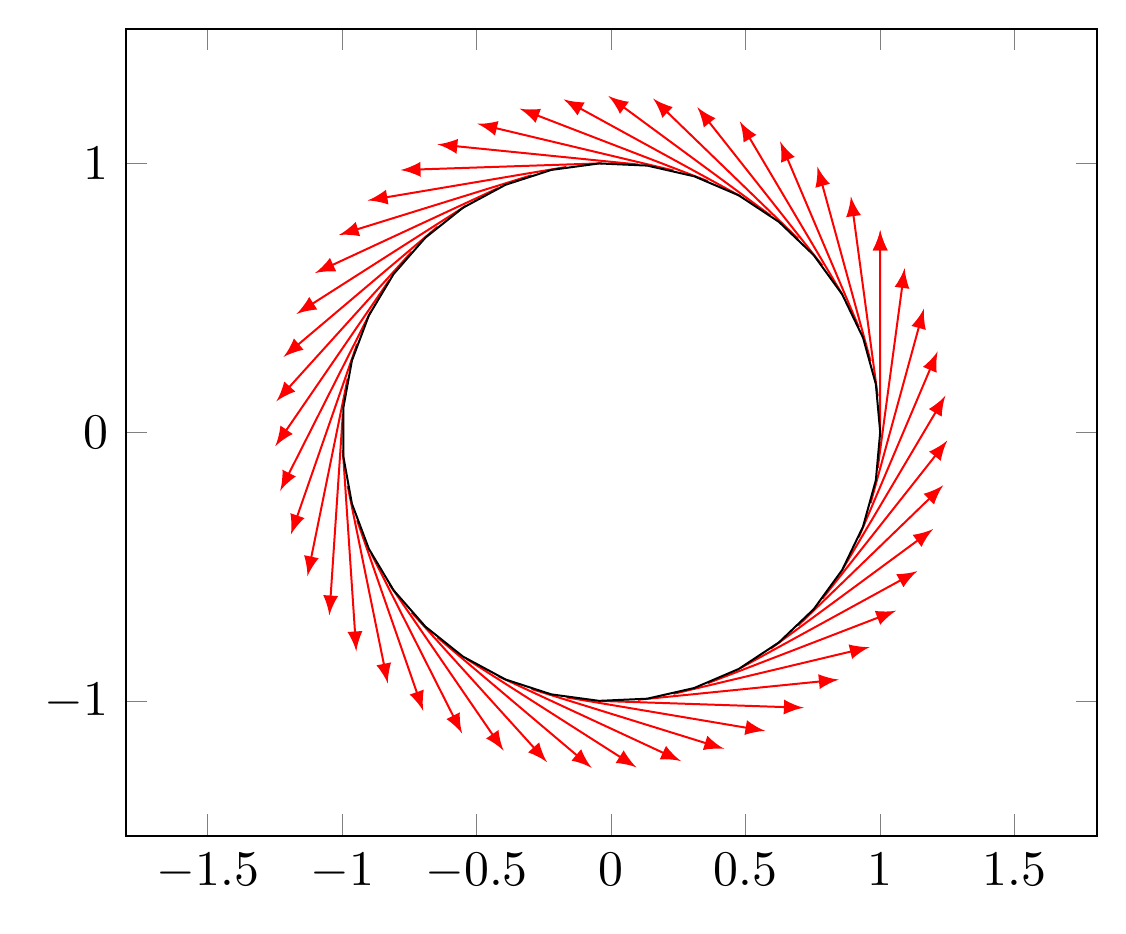
\begin{tikzpicture}[scale=1.8]
    \begin{axis}[xmin=-1.5, xmax=1.5, ymin=-1.5, ymax=1.5, axis equal]
    
        \addplot[samples=48, domain=0:2*pi, -latex, variable=\t,
            quiver={u={-sin(deg(t))},
                    v={cos(deg(t))},
                    scale arrows=0.75,
                    colored=red}]
                ({cos(deg(t))}, {sin(deg(t))});
       
        \addplot[samples=36, domain=0:2*pi]
            ({cos(deg(x))}, {sin(deg(x))});
    \end{axis}
\end{tikzpicture}
\caption{Parametrizations}
\end{figure}
\end{verbatim}
%%%%%%%%%%%%%%%%%%%%%%%%%%%%%%%%%%%





\newpage
\begin{verbatim}
\begin{figure}[ht]
\centering
\begin{tikzpicture}[scale=1.5]
    \begin{axis}[xmin=-5, xmax=5, ymin=-28, axis equal]
        
        \addplot[samples=24, domain=0:2*pi, dashed, data cs=polar,
        top color=Blues-I, bottom color=Blues-B] (deg(x),30);
        
        \addplot[name path=Y, samples=24, domain=0:2*pi, dashed, 
        data cs=polar] (deg(x),30);
        
        \addplot[GnBu-M, name path=X, domain=0:360, samples=36, smooth,
        data cs=polar] (x, {30-8*sin(3*x)});
        
        \addplot[green] fill between[of=Y and X];
        
        \addplot [samples=36,domain=0:30, dashed, data cs=cart]
        {.025*x^2} node [pos=1.1] {Node};
        
        \addplot[mark=oplus, only marks] coordinates {(0,0)};
        \node[pin=120:{Pin}] at (0,0) {};
    \end{axis}
\end{tikzpicture}
\caption{Nodes and filling}
\end{figure}
\end{verbatim}

%%%%%%%%%%%%%%%%%%%%%%%%%%%%%%%%%%%





\newpage
\begin{verbatim}
\begin{figure}[ht]
\centering
\begin{tikzpicture}[scale=1.75]
    \begin{axis}[xmin=-1, xmax=2, ymin=-3.5, ymax=1, axis equal=false]

        \addplot[red, patch type sampling, patch type= cubic spline,
        domain=0:2, smooth]{ln(x)};
        
        \draw (0,0) .. controls (1,-1.2) and (1,1) .. (2,1);
   \end{axis}
\end{tikzpicture}
\caption{Interpolation and paths}
\end{figure}
\end{verbatim}
%%%%%%%%%%%%%%%%%%%%%%%%%%%%%%%%%%%





\newpage
\begin{verbatim}
\begin{figure}[ht]
\centering
\begin{tikzpicture}[scale=1.75]
    \begin{axis}[colormap/PuBu, samples=10, domain=-4:4, y domain=-4:4,
    xmin=-4, xmax=4, ymin=-4, ymax=4, enlargelimits=false]
    
    \addplot3[surf, samples=18, samples y=36]{x^2+y^2-1};
\end{axis}
\end{tikzpicture}	
\caption{3D Surfaces}
\end{figure}
\end{verbatim}
%%%%%%%%%%%%%%%%%%%%%%%%%%%%%%%%%%%





\newpage
\begin{verbatim}
\begin{figure}[ht]
\centering
\begin{tikzpicture}[spy using outlines={}]
    \begin{axis}[xmin=-1, xmax=6, ymin=0, ymax=1,
    axis equal=false, grid=major, xtick=data, ytick=data,
    every axis plot post/.append style={thick}]

        \addplot[line join=round, green]
            coordinates {(1, 0) (1,.75) (3, 0.9) (4, .75) (5, 0.8)};
            
        \addplot[line join=bevel, blue]
            coordinates {(0, 0) (1, 0.4) (3, 0.2) (4, 1) (5, 0.9)};

        \coordinate (spypoint)     at (1,.4);
        
        \coordinate (magnifyglass) at (-2,.25);
\end{axis}
\spy[blue, size=1.5cm, circle, magnification=5, connect spies]
    on (spypoint) in node[fill=white]
                  at (magnifyglass);
\end{tikzpicture}	
\caption{Spy}
\end{figure}
\end{verbatim}

%%%%%%%%%%%%%%%%%%%%%%%%%%%%%%%%%%%





\newpage
\begin{verbatim}
\begin{figure}[ht]
\centering
\begin{tikzpicture}[scale=1.75]
	\begin{axis}[xmin=0, xmax=3.5, ymin=0, ymax=5]
	   
       \draw [name path=A] (2,3) ellipse (1.5 and 1.25);
	   
       \draw [name path=B] (1.5,1.5) rectangle (3,5);
       
       \fill [red, opacity=.5, name intersections={of=A and B}]
            (intersection-1) circle (2pt) node[above right] {1}
            (intersection-2) circle (2pt) node[above left] {2} 
            (intersection-3) circle (2pt) node[below left] {3} 
            (intersection-4) circle (2pt) node[below right] {4};
	\end{axis}
\end{tikzpicture}
\caption{Intersections}
\end{figure}
\end{verbatim}

%%%%%%%%%%%%%%%%%%%%%%%%%%%%%%%%%%%





\newpage
\begin{verbatim}
\begin{figure}[ht]
\centering
\tdplotsetmaincoords{70}{135}
\begin{tikzpicture}[scale=3, tdplot_main_coords]
    
    \tdplotsphericalsurfaceplot[parametricfill]{36}{36}
        {sqrt(15/2)*sin(\tdplottheta)*cos(\tdplottheta)}
        {black!10}{\tdplotphi};

    {\draw[color=black,thick,->] (0,0,0) -- (2,0,0) 
        node[anchor=north east]{$x$};}

    {\draw[color=black,thick,->] (0,0,0) -- (0,2,0) 
        node[anchor=north west]{$y$};}
    
    {\draw[color=black,thick,->] (0,0,0) -- (0,0,2) 
        node[anchor=south]{$z$};}
\end{tikzpicture}
\caption{Tikz-3dplot}
\end{figure}
\end{verbatim}

\newpage

\begin{appendices}               %%%%%%%%%%%%%%%%%%    (COMMENT IF NOT NEEDED)
% !TEX root = ../ArticleTemplate.tex
%%%%%%%%%%%%%%%%%%%%%%%%%%%%%%%%%%%%%%%%%%%%%%%%%%%%%%%%%%%%%%%%%%%%%%%%%%%%%%%%%%
%%%%%%%%    (APPENDICES TOC)
\addtocontents{toc}{
  \protect\vspace{25pt}
  \protect\noindent\qquad\qquad\bfseries{\Large\AppendixPart}
  \protect\par
  \protect\vspace{10pt}}

%%%%%%%%
\section*{Appendices}    %%%%%%%%%%%%%%%%%%          (DO NOT EDIT)

% !TEX root = ../../ArticleTemplate.tex
%%%%%%%%%%%%%%%%%%%%%%%%%%%%%%%%%%%%%%%%%%%%%%%%%%%%%%%%%%%%%%%%%%%%%%%%%%%%%%%%%%
\section{Title}\label{AppendixA}
	\blindduck[maths]
\end{appendices}

\newcommand\AnalyticIndexYes{0}
    %%%%%%%%%%%%%%%%%%   (IF AN ANALYTIC INDEX IS NEEDED, CHANGE 0 TO 1)
% !TEX root = ../ArticleTemplate.tex
%%%%%%%%%%%%%%%%%%%%%%%%%%%%%%%%%%%%%%%%%%%%%%%%%%%%%%%%%%%%%%%%%%%%%%%%%%%%%%%%%%
\let\clearpage\relax
%%%%%%%%%                       (BIBLIOGRAPHY PAGE FORMAT)
\fancypagestyle{fancyBibliography}{
	\renewcommand{\headrulewidth}{0.25pt}
	\renewcommand{\footrulewidth}{0.25pt}
	\fancyfoot[LE,RO]{}
	\fancyhead[LO,RE]{\bf\small \BibliographyName}}

%%%%%%%%%%                      (ANALYTIC INDEX PAGE FORMAT)
\fancypagestyle{fancyIndex}{
	\renewcommand{\headrulewidth}{0.25pt}
	\renewcommand{\footrulewidth}{0.25pt}
	\fancyhead[L,R]{}
	\fancyfoot[L,R]{}
	\fancyfoot[C]{\small\thepage}
	\fancyfoot[LE,RO]{}
	\fancyhead[LO,RE]{\bf\small \AnalyticIndexName}}

%%%%%%%%%%%%%%%%%%%%%%%%%%%%    (BIBLIOGRAPHY)
\pagestyle{fancyBibliography}
    \renewcommand{\refname}{\BibliographyName}
{
    \addcontentsline{toc}{section}{\BibliographyName}
    
	\nocite{*}
	\bibliographystyle{unsrtnat}   % Alternatives: amsalpha
    \bibliography{Structure/Bibliography}
}

%%%%%%%%%%%%%%%%%%%%%%%%%%%%    (ANALYTIC INDEX)
 \pagestyle{fancyIndex}
	\titlespacing*{\section}{0pt}{0\baselineskip}{5\baselineskip}
    \section*{\AnalyticIndexName}
    \addcontentsline{toc}{section}{\AnalyticIndexName}
\vspace{-5.5cm}
    \printindex
    \newpage    %%%%%%%%%%%%%%%%%%          (DO NOT EDIT)
\end{document}